% Chapter Template

\chapter{Comparison} % Main chapter title
\label{Chapter5} % Change 5 to a consecutive number; for referencing this chapter elsewhere, use \ref{Chapter5}

A lot of companies and individual developers are torn between which framework or library to choose for developing client-side applications. ReactJS and Angular are the two most popular choices used for this purpose. In this chapter, these two technologies will be compared based on both personal experiences and what has already been analyzed in previous Chapters. \par

There are no official references or scientific papers citing the comparison of ReactJS and Angular so far. For this reason, personal experience in both technologies will be the guide. As regards my experience, I have created a complete web application in Angular7 which is called \href{https://snf-844240.vm.okeanos.grnet.gr/#/index}{Hom-e} and is a home aggregator, while I was coding in React during my internship. \par

Chapter \ref{Chapter5} includes six main sections that will form the key points of comparison. Firstly, architectural differences based on previous Chapters are pointed out. Moreover, mobile application choices, testing capabilities, learning curve, performance and popularity of each technology will be cited. In the end, a discussion about the topic and a recap are included. \par

\section{Architectural Differences}

Based on Chapters \ref{Chapter2}, \ref{Chapter3} and \ref{Chapter4}, architectural differences of ReactJS and Angular will be pointed out. This section is separated into seven main parts. \par

\subsection{Framework \& Library}

One of the main differences of ReactJS and Angular is that the one is a JavaScript library that provides only the view layer, while the other is a complete MVC framework that provides all functionality needed to the app. \par

As regards Angular, it is a framework. As mentioned in Chapter \ref{Chapter2} and \ref{Chapter4}, frameworks provide a collection of libraries and functions to support most features needed in an application. Angular apps have a defined way of how their structure is. Developers do not need to spend time deciding which extended libraries to use, such as routing libraries, but they can directly start coding. However, there is less flexibility since they need to use what Angular provides. \par

On the other hand, ReactJS is a user interface component library. This means that it does not aim to provide a complete solution for developing a client-side application, as it is also referred to Chapter \ref{Chapter3}. The React library provides the view implementation, while external libraries are needed for adding functionality in the application. This leads to freedom of choice comparing to Angular, but also many more dependencies. When using ReactJS, developers need to upgrade and migrate dependencies. Furthermore, the architecture and folder hierarchy of each React project differs. Thus, the app's performance and maintainability can be affected to a large extent. \par

\subsection{Real \& Virtual DOM}

In Chapter \ref{Chapter3}, we mentioned that ReactJS is using virtual DOM instead of the actual one. This is because virtual DOM can be accessed and changed faster than real DOM which is on the browser's memory. In more detail, React's DOM is used as another instance of DOM and all changes needed are first made in that. When all changes are applied, the differences between previous and current HTML are checked, and only the updated parts of the tree are applied in real DOM. This results in higher performance and speed of React apps. (\cite{Reference6}) \par

Contrarily, Angular is applying changes directly to Real DOM. More specifically, Angular is first detecting changes made for each component, and then it rules how those will enter to DOM. A change detector is applied for each component of the application. Detectors are responsible for recognizing updates made inside the component and then modifying DOM only at its changed parts. By using detectors, Angular is fast, but for higher speed, Immutables and Observations are used. Through Immutables, checks to each property are reduced, while through Observables, events are triggered and change detection is limited to specific properties. (\cite{Reference6}) \par

\subsection{Templates: HTML \& JSX}

React is using JSX syntax as shown in Chapter \ref{Chapter3}, which is a combination of UI templates and inline JS logic. In this way, components used in React include both markup and logic in the same file. For this reason, a lot of developers think that having everything in one place results in code completion and compiling checks. Regarding Angular, as referred to Chapter \ref{Chapter4}, it uses templates that are HTML embellished with directives, such as "ng-if" for attaching custom behavior to DOM. \par

\subsection{TypeScript \& JS}

In Chapter \ref{Chapter3}, it was mentioned that React developers mostly write in JavaScript to add functionality in their application. JS is a dynamically-typed language, meaning that variables do not need to be defined. JavaScript also includes lots of useful features to its early versions (up to ES6) that lead to stating coding and a class-based structure. React favored by Flow, static checker developed by Facebook, supports checking of types as well. \par

Controversially, based on Chapter \ref{Chapter4}, Angular is mostly used alongside with TypeScript, a typed JavaScript-based language that transpiles into JS code. TypeScript's advantage is its typing system that can prevent developers from bugs and unreadable code. It was firstly developed for providing an Object-oriented structure to JavaScript developers before the induction of ES6. \par

Based on my experience, lots of developers prefer writing in JavaScript, since is widely used and doesn't limit quick developers with a typing system, like TypeScript. TypeScript has its own rules and quick coding is not an easy choice, but it prevents from compiling-time errors. \par

\subsection{Components}

Both React and Angular are using components to their structure. Components are JavaScript functions that take inputs named properties, revise those inputs and return as output UI elements, which are what a user sees. It is a good practice to work in components since they are small reused parts of the code that reduce complexity and enhance the maintainability of code. \par

\subsection{State Management}

In an application, every component has its state. More specifically, the state is an interval store in which variables of any type can be saved and used inside the component. \par

In React, Redux is usually adopted for the app's state management, as referred in Chapter \ref{Chapter3}. Redux is providing global storage that any component can access if needed. This is how the interaction between components is succeeded. \par

In Angular, state management is handled by the framework. However, as the application goes larger, the state is not easily managed, and Redux can be used for components' connection as well. \par

\subsection{Data Binding}

One main difference between ReactJS and Angular is how they manage data. In Angular's Chapter (\ref{Chapter4}), it is mentioned that Angular used to have two-way data binding, meaning that data flow from state to view and vice versa. Even if this approach seems to be simple, it is possible to cause unpredictable updates and difficulties of following data flow, as the application goes bigger. By adding more and more logic, different views update the same models which can also update other views, a fact that can cause an infinite loop problem. (\cite{reactQuickly}) In this way of binding data, event handlers are not needed, but they are managed by Angular. Nowadays, in new versions of React developers have also the choice of one-way data binding by adding either Observables or libraries like Redux. \par

In React, there is a one-way data flow, which means that only the state can update user interface elements and not the other way around. As mentioned in Chapter \ref{Chapter3}, React is well combined with Redux, a state management library following a one-way data flow. Thus, there is better data overview, a fact that leads to easier debugging. \par

Both approaches have advantages and disadvantages. Though, when it comes to large and complex projects, two-way data binding causes slow manageability and performance. Controversially, one-way data binding leads to easier handling and maintainable data flow, since event handlers are managed by developers and thus each phase of components' state is known. \par

\section{React Native \& IONIC}

Both React and Angular can be used for building mobile applications. More specifically, React uses the so-called React Native. React Native is a platform developed by Facebook and uses JavaScript, declarative components and the same design as React. React and React Native have small differences in syntax since the second one is using the same user interface blocks as iOS and Android apps. (\cite{Reference16}) \par

On the other hand, the Ionic Framework can be integrated with Angular for the development of mobile applications. Ionic Framework is an open source UI tool for building hybrid applications based on web technologies, such as HTML, CSS, and JS. Ionic has official incorporation with Angular but it also supports other libraries like React and Vue. (\cite{Ionic}). \par

It has to be mentioned that Ionic-based mobile apps are just web applications inside a native view container, and not truly native as React Native is. Thus, comparing to React Native, Ionic apps are slower and with lower performance. \par

\section{Testing}

As regards testing, Angular is providing Angular CLI that is a command-line interface for creating apps and adding files, tests and deployment capabilities, like it was analyzed in Chapter \ref{Chapter4}. Moreover, Angular can be integrated with other end-to-end testing and debugging tools, such as Jasmine, Karma, and Protractor. \par

On the other hand, React is using Jest, a library created by Facebook for JavaScript code testing. Jest is included in every React app and is well integrated with Enzyme for component testing. A drawback of React is that it uses lots of separate tools for different types of testing, such as Jest for JS code, Enzyme for components, a react-testing library for Virtual DOM testing, react-unit for unit testing and skin-deep for render testing. \par

\section{Learning Curve}

When it comes to choosing new technology for building web apps, an important parameter is its learning curve. The learning curve depends on the developer's previous knowledge and familiarity with the discussed technology. In this section, we will point out what it is needed to be known when developing in React and Angular. \par

For building React applications, it is needed to learn how to code in JSX, create components and manage state. It is also needed to write JavaScript for adding logic in the app. If a developer knows how to code in JS, React's development becomes much easier. Furthermore, React doesn't include any routing capabilities, which may be both pro and con in terms of learning. Developers can choose their preferred rooting library, but if they are not familiar with any, this is a plus in learning features. Redux is also another library that most React users need to learn since it provides state management. In general, React is not the most simple choice, because of the additional libraries and JSX. However, due to its flexibility, it is considered to be simpler than a framework (\cite{reactQuickly}). \par

Angular is a framework which means that has its ways of handling things, such as installation, error messages and compilation. Directives, modules, state management, decorators, services, components, dependency injection, template, and pipes are some additional features of Angular that need developers' attention. Angular may have the biggest learning curve because of TypeScript, specifically for those who are not familiar with JavaScript frameworks (\cite{Reference6}). \par

\section{Performance}

Application's performance is an important criterion of choosing between ReactJS and Angular, because of responsiveness and user experience. To compare these two technologies' performance, technical factors that are based on the application's execution phases will be mentioned. More specifically, these factors are the startup time of the app and the DOM's creation and modification. Even though these two are depending on the user's browser, and its JavaScript engine, supporting different types of browsers and application's performance in each of them is also considered. \par

In React applications, startup time is relevant to what libraries are added in the app. React do not have many dependencies, unlike a framework, cause most of the features needed are included as dependencies. Thus, if there are not many external libraries, the package size is smaller and the performance is higher. Moreover, React can also include routing libraries that are dividing JavaScript content into parts. In this way, these parts are fetched from servers based on page changes, a fact that limits loading time as well. Furthermore, React's virtual DOM, as mentioned before, is designed for improving performance and user experience. (\cite{Reference6}) \par

As regards Angular, as being a framework includes lots of libraries that may not be needed, so performance is reduced comparing to React. Though, its impeded routing library, separate code into parts that are loaded asynchronously when it is needed. One more thing that improves the performance of Angular apps is TypeScript's compilation. TypeScript can select between Just-in-time compilation, in which HTML elements are compiled in the browser and output can be seen directly, and Ahead-of-time compilation, in which HTML elements are compiled in the server and in this way, rendering is faster in a browser. (\cite{Reference6}) \par

\section{Popularity}

Popularity is one of the key ways to choose across new technology since it considered to be the measure of community support and so to the effectiveness of the application's development. This section's purpose is to examine ReactJS and Angular's popularity according to GitHub, Google trends, npm trends, and what well-known companies have chosen to use. \par

GitHub is a company and provides hosting for software development version control through Git. Both ReactJS and Angular are open-source and their code can be found in their respectively public repositories. Stars on GitHub is a way for GitHub's users to favor the most useful and used repositories. \href{https://github.com/angular/angular}{Angular's repository} has, at the time this thesis was written, 49,250 stars, 13,411 forks, and 954 contributors, while there are 2,496 issues due to framework's variety of functionalities. On the other hand, \href{https://github.com/facebook/react/}{React's repository} has 131,625 stars, 24298 forks, and 1,298 contributors, and as a library only 556 issues. React seems to be much more popular based on GitHub stars and contributors, but we need to take into account that Angular (up to version 2) was released 3 years later than React. \par

Another good metric is the number of downloads made. For this purpose, we used npm trends for comparing downloads during the past two years in both ReactJS and Angular. As figure 5.1 reveals, two years ago React and Angular had approximately the same number of downloads, while now react has 3,870,000 more. 

\begin{figure}[H]
	\begin{center}
		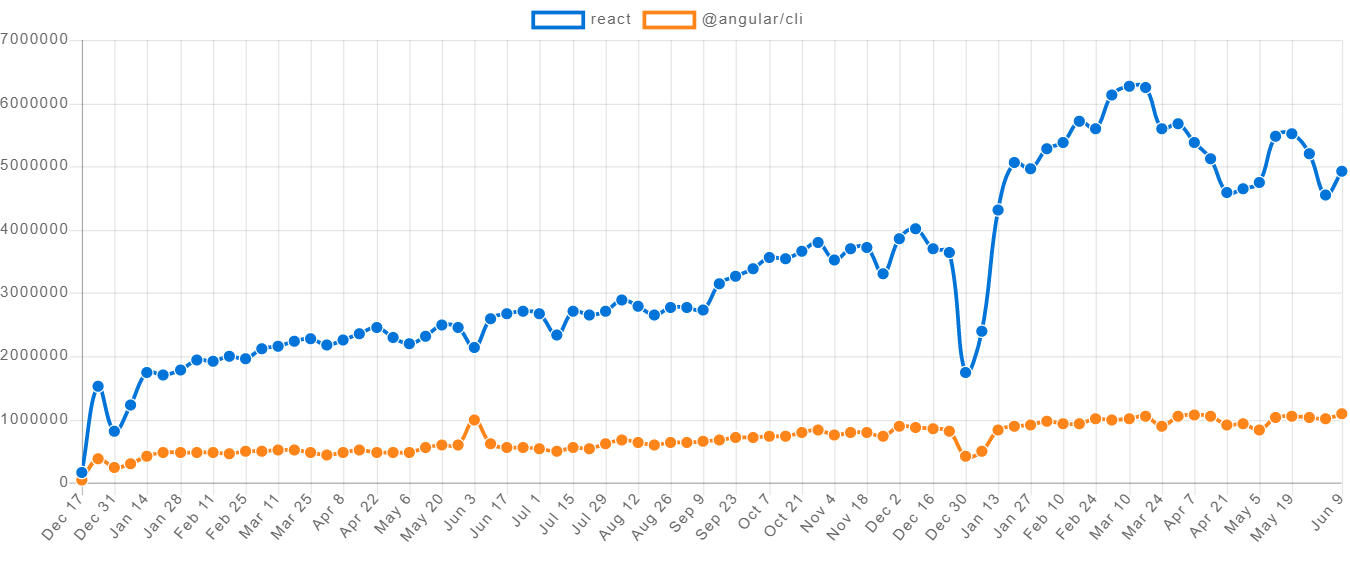
\includegraphics[scale=0.3]{images/npm-trends-react-vs-angular.png}
	\end{center}
	\caption{
		Npm trends of ReactJS and Angular CLI
		\\
		\textbf{Source:} \url{https://www.npmtrends.com/react-vs-@angular/cli}
	}
\end{figure}

Furthermore, the Google Trends search hit is another way of measuring popularity. According to Google Trends's chart, Angular, which is the red line, used to be more searched worldwide in Google's search engine two years ago. Nowadays, React seems to win with 30 more hits on average every day. In figure 5.2 (B), it is shown that in China and North America is mostly used to React library, while in Latin America and some European countries Angular framework.

\begin{figure}[H]
	\centering
	\subfloat[Trends during 16/06/2015-2019]{{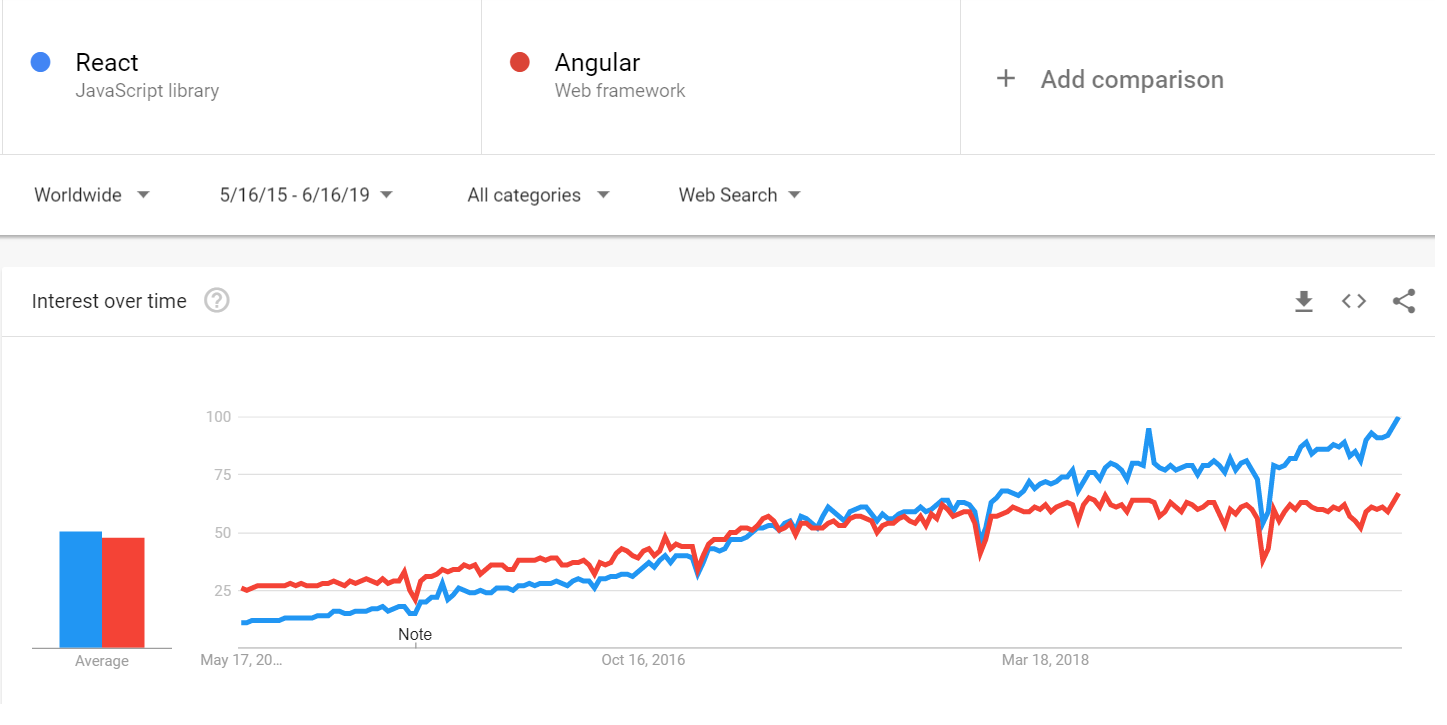
\includegraphics[scale=0.2]{images/ReactJS-VS-Angular-Google-Trends.png} }}%
	\qquad
	\subfloat[Countries' preferences]{{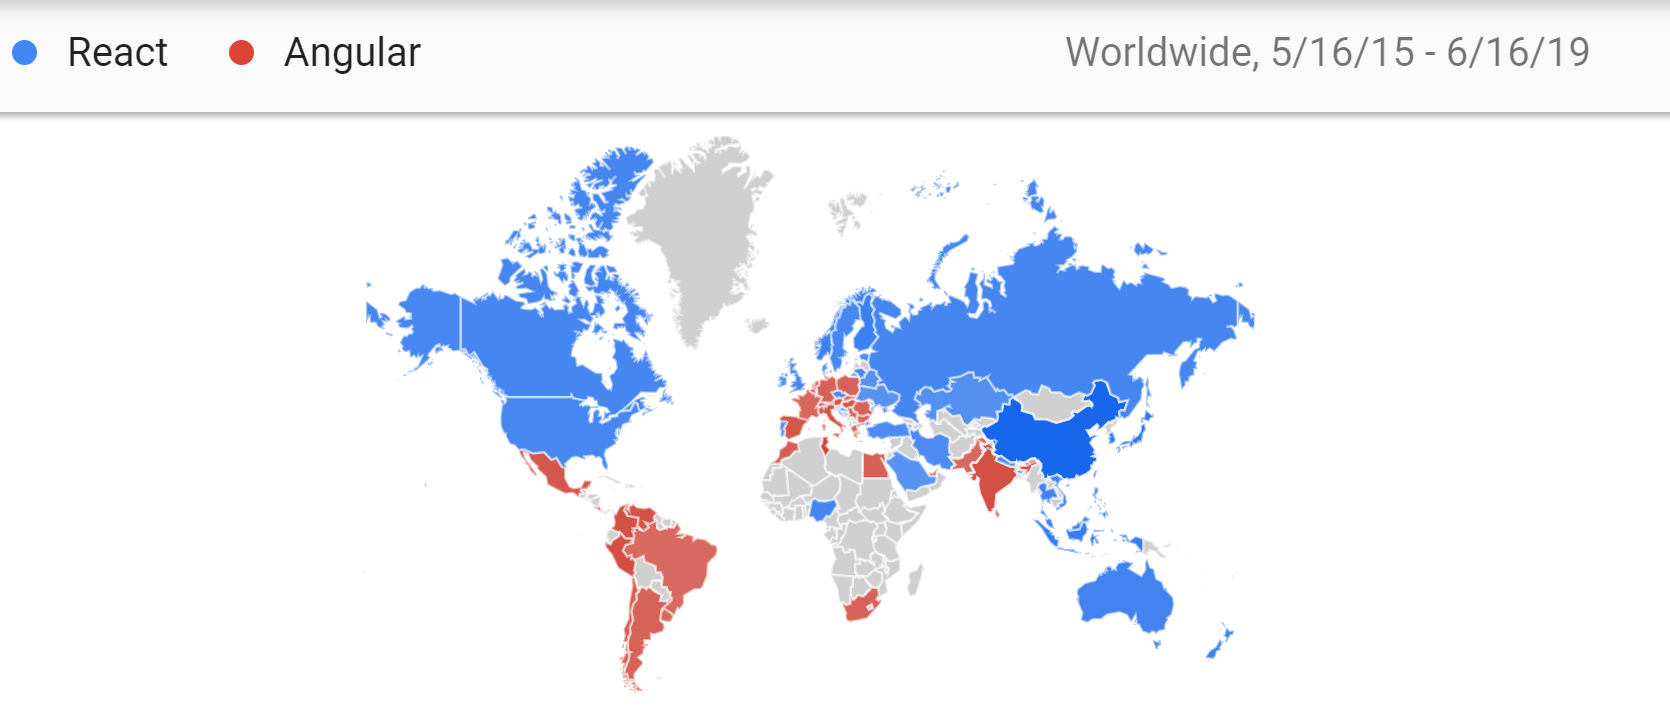
\includegraphics[scale=0.2]{images/ReactJS-VS-Angular-Google-Trends-Map.png}}}%
	\caption{
		ReactJS VS Angular in Google Trends
		\\
		\textbf{Source:} \url{https://trends.google.com/trends/explore?date=2015-05-16\%202019-06-16\&q=\%2Fm\%2F012l1vxv,\%2Fg\%2F11c6w0ddw9}
	}
	\label{fig:example}
\end{figure}

Based on the previous metrics, React seems to grow faster than Angular does. However, both technologies are pretty popular among professional developers, as indicated in Stackoverflow's survey in 2019. 

\begin{figure}[H]
	\begin{center}
		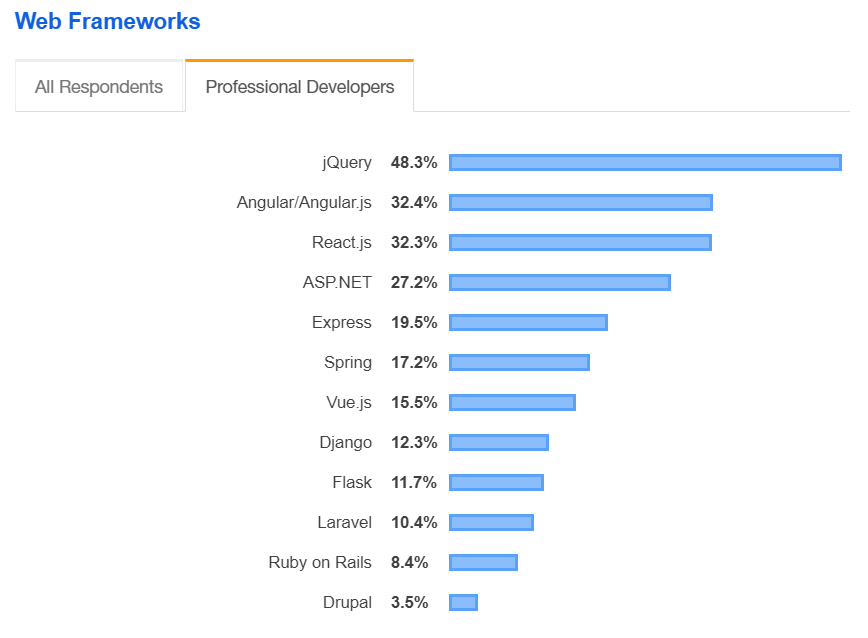
\includegraphics[scale=0.5]{images/ReactJS-VS-Angular-Survey-Stackoverflow.png}
	\end{center}
	\caption{
		ReactJS-VS-Angular Survey Stackoverflow 2019
		\\
		\textbf{Source:} \url{https://insights.stackoverflow.com/survey/2019}
	}
\end{figure}

\subsection{What are companies using?}
There are a lot of companies that utilize both ReactJS and Angular to their applications. Some of the most famous ones in React development are Facebook, Airbnb, Uber, Netflix, Instagram, WhatsApp, and Dropbox. Other known companies that are using Angular instead are Google, Nike, Forbes, Upwork, General Motors, HBO and Sony.

\section{Discussion}

During my internship, I experienced some good practices and problems as a new developer to React that can be compared to Angular. First of all, it is good practice to use Redux. State mismanagement can lead to complex apps and unresolved bugs. Redux is using a global state, through which interaction between components is succeeded, and it leads to one-way data flow via selectors and actions usage. \par

Furthermore, in many cases, I had to use React's life-cycle methods to complete and improve the functionality of features added in BeatHotel's web application. Through these methods, it is possible to execute code and update state in specific phases of component.\par

Additionally, another good practice is the usage of ES6 instead of ES5 JavaScript. ES6 is providing many more features, such as arrow functions, stating code and an object-oriented approach that improves coding. In my point of view, Angular's TypeScript is not that easy to be handled but prevents developers from bugs and compile-errors. \par

On the other hand, a great problem of React apps is the difficulty of upgrading the project, due to the variety of dependencies added. A lot of dependencies are using other libraries. This means that when a dependency is upgraded, the project may crash if its required libraries are not updated as well. Controversially, Angular handles automatically its upgrades, since most of the libraries used are embedded in the framework. \par

Both Angular and ReactJS have advantages and disadvantages. When it comes to choosing between the two, there have to be considered metrics regarding the development team’s previous experience, library/framework's popularity, performance and other capabilities like mobile application development or testing. \par
